\documentclass[a4paper]{article}
\usepackage[affil-it]{authblk}
\usepackage[backend=bibtex,style=numeric]{biblatex}
\usepackage{graphicx}
\usepackage{amsmath}
\usepackage{geometry}
\usepackage{listings}
\usepackage{array}
\usepackage{tcolorbox}
\usepackage{booktabs}
\usepackage{float}
\geometry{margin=1.5cm, vmargin={0pt,1cm}}
\setlength{\topmargin}{-1cm}
\setlength{\paperheight}{29.7cm}
\setlength{\textheight}{25.3cm}



\begin{document}
% =================================================
\title{Numerical Analysis  programming homework \# 2}

\author{Liang Yuwei 3230102923
  \thanks{Electronic address: \texttt{liangyuwei631@gmail.com}}}
\affil{(Mathematics and Applied Mathematics 2302), Zhejiang University }


\date{\today}

\maketitle

\begin{abstract}
  This report presents the design and implementation of interpolation algorithms, including Newton's interpolation, Hermite interpolation, and Bezier interpolation. The Runge phenomenon is discussed, and the Chebyshev interpolation method is applied to mitigate the issue. The Hermite interpolation algorithm is used to solve a problem involving a car's position and velocity. The interpolation algorithms are applied to fit data on larvae survival, and the cubic spline interpolator and exponential fitting are used to improve the results. Finally, the Bezier interpolation algorithm is used to fit a planar curve.
\end{abstract}

% ============================================
\section{A. Interpolator Design}

\subsection{Class Structure and Inheritance}
The \textbf{Interpolator} class serves as a base class, which is inherited by the derived classes \textbf{NewtonInterpolator} and \textbf{HermiteInterpolator}.\\
As in problem F, the interpolation object is a point. Therefore, I designed the \textbf{Point} class and another base class, \textbf{PointInterpolator}, which is inherited by \textbf{BezierInterpolator}.

\subsection{Newton Interpolator}
The \textbf{NewtonInterpolator} class is derived from the \textbf{Interpolator} base class. It is designed to perform Newton's interpolation. The class has two constructors and several member functions.

The first constructor takes two vectors, \texttt{x\_values} and \texttt{f\_values}, which represent the x-coordinates and corresponding function values, respectively. It initializes the divided differences table and calls the \texttt{computeDividedDifferences()} function to compute it.

The second constructor takes a function object and a vector of x-coordinates. It evaluates the function at each x-coordinate to obtain the corresponding function values and then initializes the divided differences table.

The \texttt{interpolate()} function performs the interpolation for a given x-value using the precomputed divided differences.

The \texttt{printInternalData()} function prints the internal data, including the x-values and the main dialog of divided differences table.

The \texttt{computeDividedDifferences()} function computes the divided differences table. The following is the pseudocode:
\begin{lstlisting}
for i = 0 to n
    dd[i][0] = f[i]
for j = 1 to n
    for i = j to n
        dd[i][j] = (dd[i][j-1] - dd[i-1][j-1]) / (x[i] - x[i-j])
\end{lstlisting}

\subsection{Hermite Interpolator}
The \textbf{HermiteInterpolator} class is derived from the \textbf{Interpolator} base class. It is designed to perform Hermite interpolation, which takes into account both function values and their derivatives at given points. The class has a constructor and several member functions.

For simplicity of design, I only considered the case where all interpolation points have first derivatives and no higher-order derivatives, which meets the requirements of problem D.

The constructor takes three vectors of \texttt{same size}: \texttt{x\_values}, \texttt{y\_values}, and \texttt{yDerivative\_values}. It initializes the divided differences table and calls the \texttt{computeCoefficients()} function to compute it.

The \texttt{interpolate()} function performs the interpolation for a given x-value using the precomputed divided differences.

The \texttt{printInternalData()} function prints the internal data, including the x-values and the main dialog of divided differences table.

The \texttt{computeCoefficients()} function computes the divided differences table. The following is the pseudocode:
\begin{lstlisting}
n = x.size()
z = new array of size 2*n
for i = 0 to n-1
  z[2*i] = x[i]
  z[2*i + 1] = x[i]
  dd[2*i][0] = y[i]
  dd[2*i + 1][0] = y[i]
  dd[2*i + 1][1] = yd[i]
  if i > 0
    dd[2*i][1] = (y[i] - y[i-1]) / (x[i] - x[i-1])
for j = 2 to 2*n-1
  for i = j to 2*n-1
    dd[i][j] = (dd[i][j-1] - dd[i-1][j-1]) / (z[i] - z[i-j])
\end{lstlisting}

\subsection{Bezier Interpolator}
The \textbf{BezierInterpolator} class is derived from the \textbf{PointInterpolator} base class. It is designed to perform cubic Bezier interpolation. The class has a constructor and several member functions.

The constructor takes a vector of control points sets, where each set contains exactly four points. It initializes the control points sets and checks if they are valid. If any set does not contain exactly four points, an exception is thrown.

The \texttt{Interpolate()} function performs the interpolation for a given parameter \( t \) in the range \([0, 1]\). It first determines the appropriate segment for the given \( t \) and maps \( t \) to the local range \([0, 1]\) within that segment. It then calls the \texttt{calculateBezierPoint()} function to compute the interpolated point.

The \texttt{calculateBezierPoint()} function computes the Bezier point for a given set of control points and a parameter \( t \). It uses the cubic Bezier formula:
\[
\mathbf{P}(t) = (1-t)^3 \mathbf{P}_0 + 3(1-t)^2 t \mathbf{P}_1 + 3(1-t) t^2 \mathbf{P}_2 + t^3 \mathbf{P}_3
\]
where \(\mathbf{P}_0, \mathbf{P}_1, \mathbf{P}_2, \mathbf{P}_3\) are the control points.

\section{B. Runge Phenomenon}
First, I implemented the Runge function \( f(x) = \frac{1}{1 + x^2} \) and computed the interpolating polynomials. Then, I plotted the function and its interpolating polynomials in the range \([-1, 1]\) using Python. The resulting plot is shown in Figure \ref{fig:runge}.
\begin{figure}[ht]
    \centering
    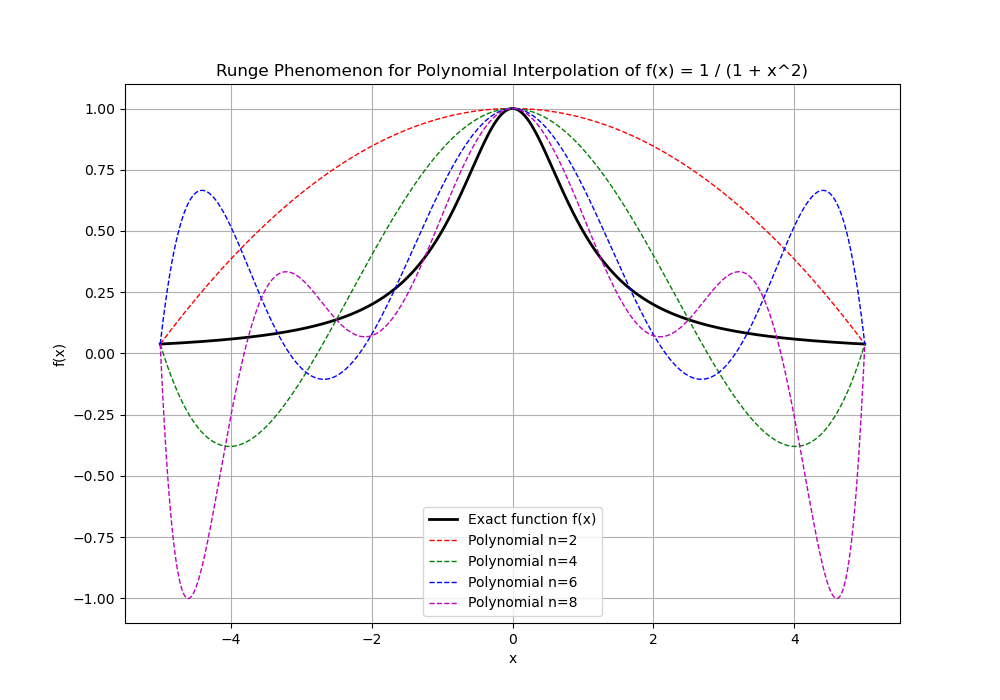
\includegraphics[width=0.6\textwidth]{figures/Runge.png}
    \caption{Runge Phenomenon}
    \label{fig:runge}
\end{figure}

From the plot, we can observe that the interpolating polynomials exhibit oscillations near the endpoints of the interval \([-1, 1]\) and do not converge uniformly to the function.

\section{C. Chebychev Interpolate}
First, I generate the Chebyshev nodes in the interval \([-1, 1]\) and evaluate the Runge function at these nodes. Then, I perform Newton's interpolation using the Chebyshev nodes and plot the interpolating polynomial. The resulting plot is shown in Figure \ref{fig:chebyshev}.
\begin{figure}[ht]
    \centering
    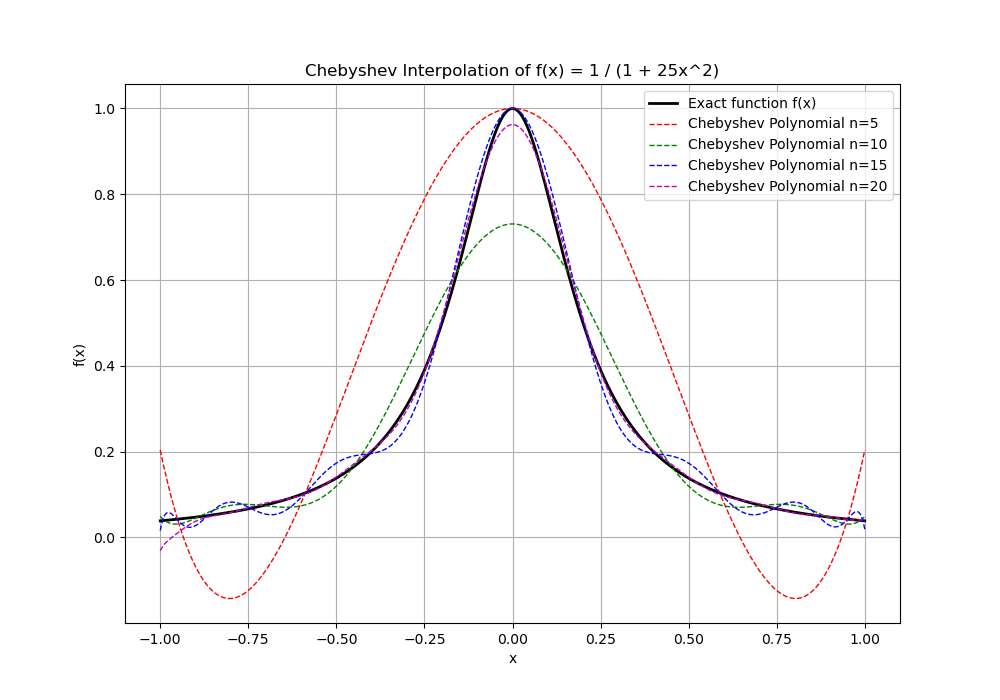
\includegraphics[width=0.6\textwidth]{figures/Chebyshev.png}
    \caption{Chebyshev interpolation}
    \label{fig:chebyshev}
\end{figure}

From the plot, we can observe that the interpolating polynomial using Chebyshev nodes exhibits less oscillation near the endpoints of the interval \([-1, 1]\) compared to the interpolating polynomial using equidistant nodes.

\section{D. Hermite Interpolation}
I implemented the Hermite interpolation algorithm and following is the result:
\begin{lstlisting}
  (a) The position at t = 10 seconds: 712.774 feet
  (b) The maximum velocity is 81.2615 feet/second, reached at t = 6.678 seconds
   The maximum velocity exceeds 81 feet/second
\end{lstlisting}
In the second question, I use the secant to subtitute the slope of the function, in other words, I use mean velocity to subtitute velocity. And by Langrange mean value theorem, we can know that the car reached 81.2615 feet/second at some moment between 6.678 and 6.679 seconds.

\section{E. larvae survival}
First, I try to use Newton interpolation to fit the data. The result is shown in Figure \ref{fig:larvae28} and Figure \ref{fig:larvae43}.
\begin{figure}[ht]
  \centering
  \begin{minipage}[b]{0.45\textwidth}
    \centering
    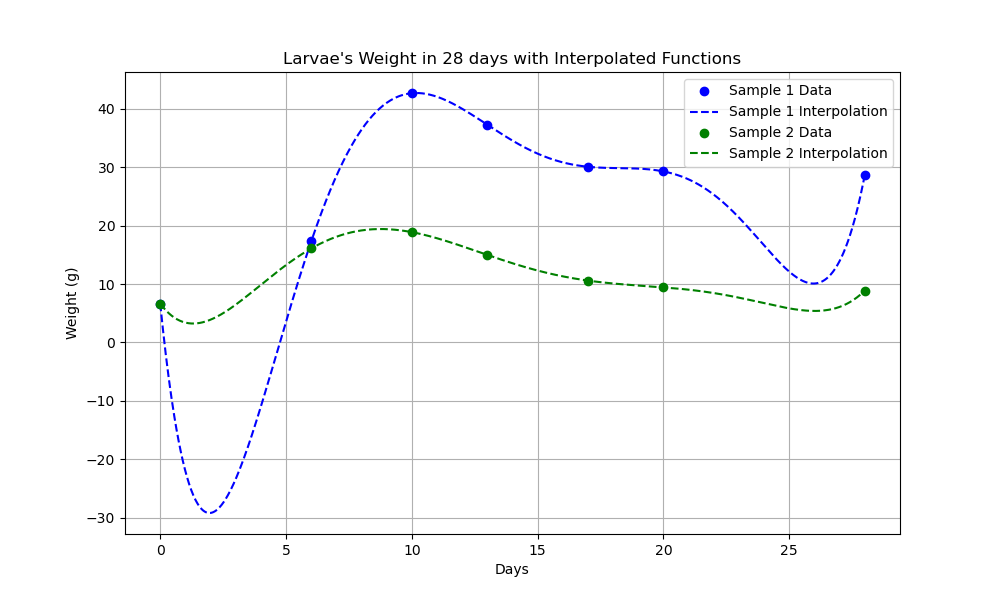
\includegraphics[width=\textwidth]{figures/larvae28days.png}
    \caption{Larvae's weight in 28 days with Newton interpolation}
    \label{fig:larvae28}
  \end{minipage}
  \hfill
  \begin{minipage}[b]{0.45\textwidth}
    \centering
    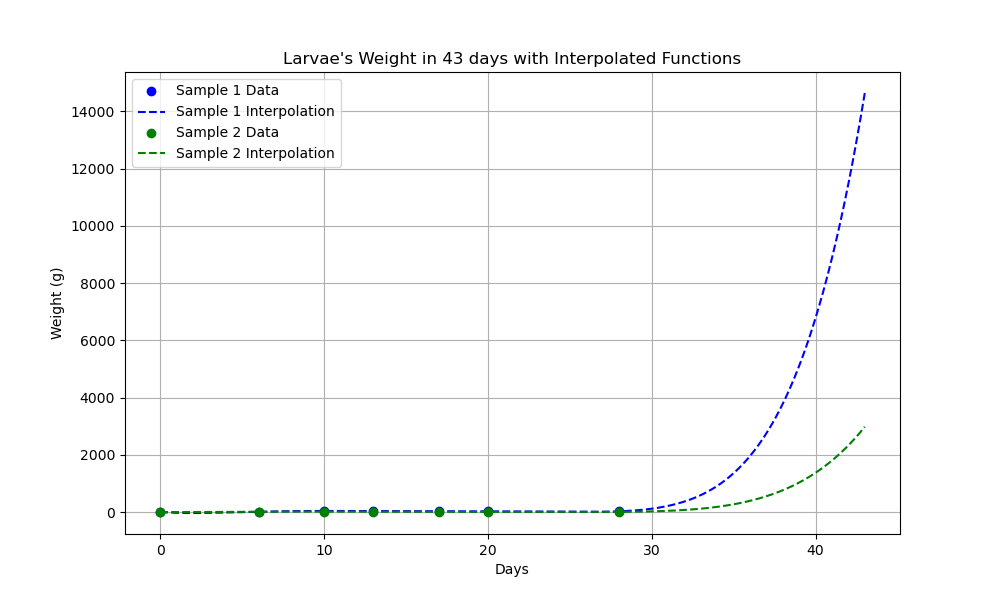
\includegraphics[width=\textwidth]{figures/larvae43days.png}
    \caption{Larvae's weight in 43 days with Newton interpolation}
    \label{fig:larvae43}
  \end{minipage}
  \vfill
  \begin{minipage}[b]{0.45\textwidth}
    \centering
    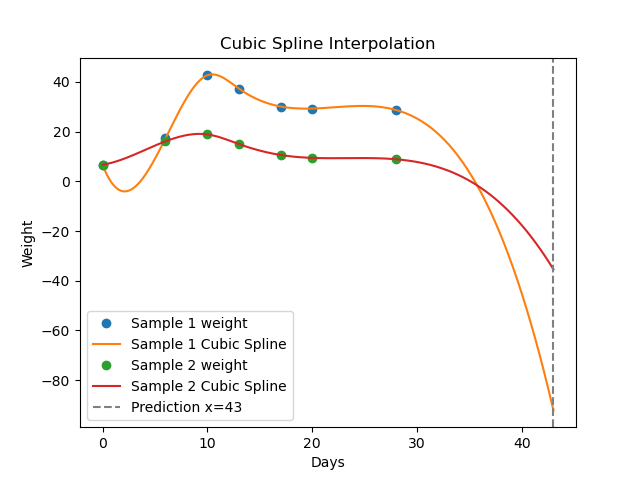
\includegraphics[width=\textwidth]{figures/cubicspline.png}
    \caption{Larvae's weight in 43 days with cubic spline interpolation}
    \label{fig:larvaeCubicSpline}
  \end{minipage}
  \hfill
  \begin{minipage}[b]{0.45\textwidth}
    \centering
    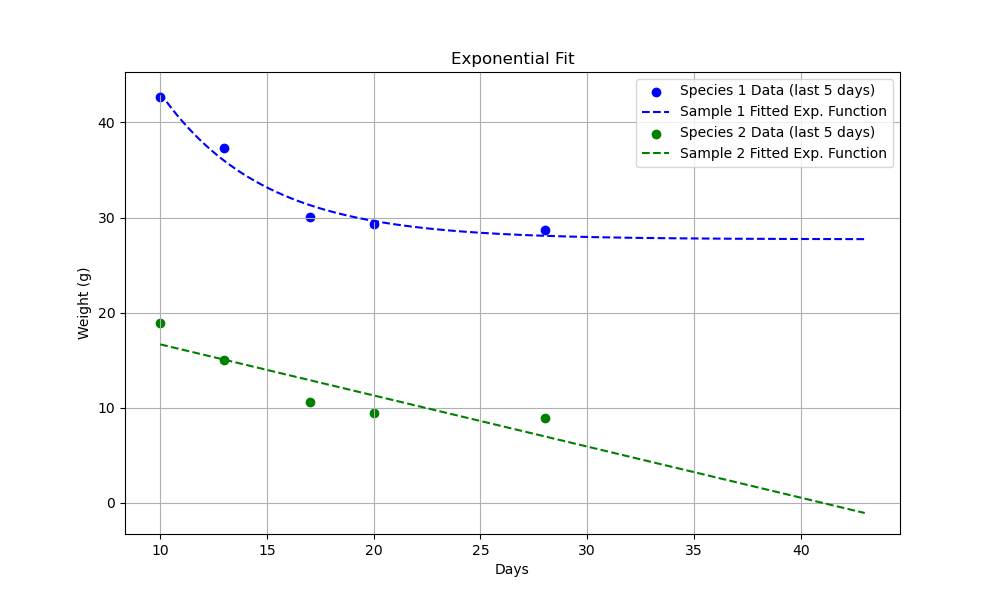
\includegraphics[width=\textwidth]{figures/expfit.png}
    \caption{Exponential fitting}
    \label{fig:expfit}
  \end{minipage}
\end{figure}

From Figure \ref{fig:larvae28}, we can observe that overfitting occurs, and sample 1 even shows negative weight values in the first five days.

In Figure \ref{fig:larvae43}, we can see that weight in 43 day shows in even greater deviations. This is because we should not use interpolation polynomials to estimate points beyond the range of our data.

To fix this, I tried to use the cubic spline interpolator, and the result is shown in Figure \ref{fig:larvaeCubicSpline}. It is much better than the Newton interpolator, but it still shows some problems.

Finally, I found that the last part of the data can be better fitted using an exponential function plus a constant, as shown in Figure \ref{fig:expfit}. This method provides a better fit for the data, leading us to conclude that sample 1 will not die in 43 days, while sample 2 will.

Unfortunately, I did not implement the cubic spline interpolator and exponential fit in this homework. These parts of the code were generated using Python with the assistance of ChatGPT-4.
\section{F. Bezier Interpolation}
First, I noticed that the function graph of the planar curve is symmetric about the y-axis, so I only considered the part where \( x \geq 0 \) during interpolation, and then obtained the entire planar curve through symmetry. At this point, the equation of the function can be simplified to \( x^2 + \left(\frac{3}{2}y - \sqrt{x}\right)^2 = 3 \).

To correctly use Algorithm 2.74, I first parameterized the points on the planar curve:
\[
\begin{cases}
  x = \sqrt{3} \sin(\pi t), \\
  \frac{3}{2}y - \sqrt{x} = \sqrt{3} \cos(\pi t)
\end{cases}
\implies
\begin{cases}
  x = \sqrt{3} \sin(\pi t), \\
  y = \frac{2}{3} \left( \sqrt{3} \cos(\pi t) + \sqrt{x} \right)
\end{cases}
\]
where \( t \in [0, 1] \).

Taking the derivatives, we get:
\[
\begin{cases}
  \frac{dx}{dt} &= \sqrt{3} \cos(\pi t), \\
  \frac{dy}{dt} &= -\frac{2}{3} \left( \sqrt{3} \sin(\pi t) + \frac{1}{2\sqrt{x}} \frac{dx}{dt} \right).
\end{cases}
\]

Then I obtained the control points using Algorithm 2.74, including the characteristic points \((0, \pm \frac{2}{\sqrt{3}})\). The results for diffenrent \(m\) are shown in following figures, while Figure \ref{fig:planar curve} is the original curve.
\begin{figure}[ht]
  \centering
  \begin{minipage}[b]{0.45\textwidth}
    \centering
    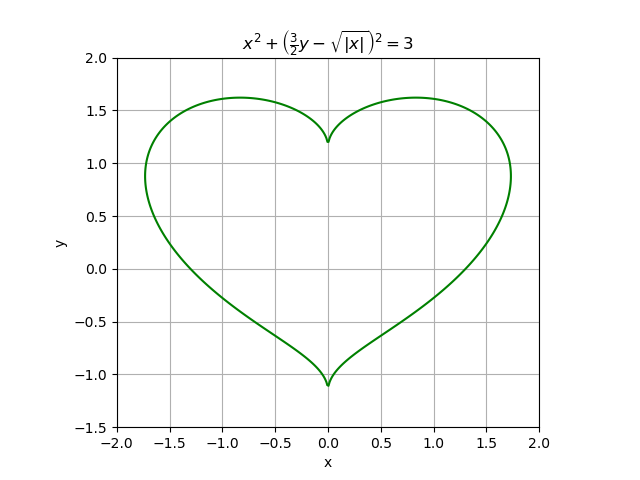
\includegraphics[width=\textwidth]{figures/bezier0.png}
    \caption{planar curve}
    \label{fig:planar curve}
  \end{minipage}
  \hfill
  \begin{minipage}[b]{0.45\textwidth}
    \centering
    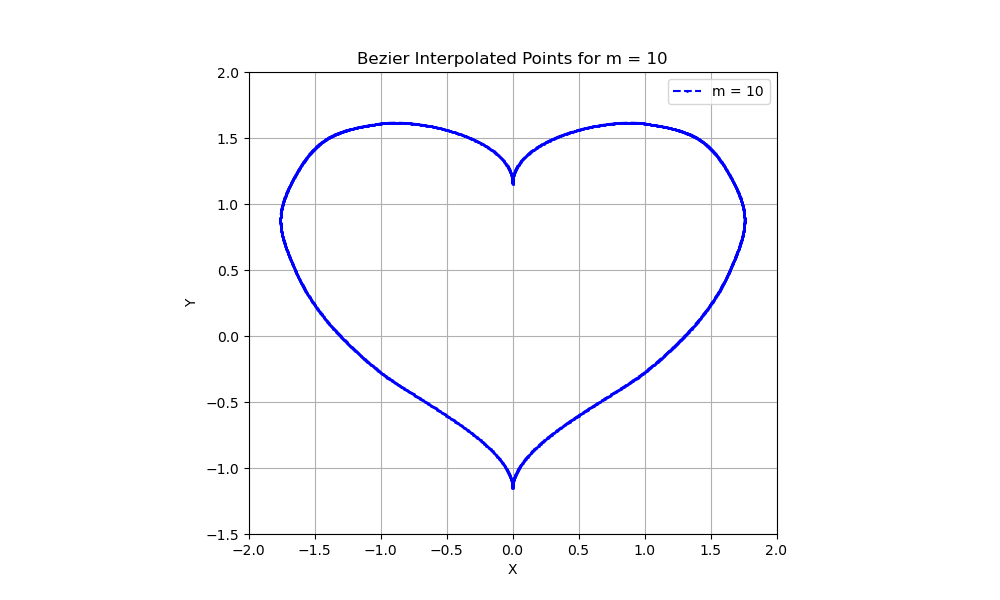
\includegraphics[width=\textwidth]{figures/bezier1.png}
    \caption{planar curve with m = 10}
    \label{fig:bezierm10}
  \end{minipage}
  \vfill
  \begin{minipage}[b]{0.45\textwidth}
    \centering
    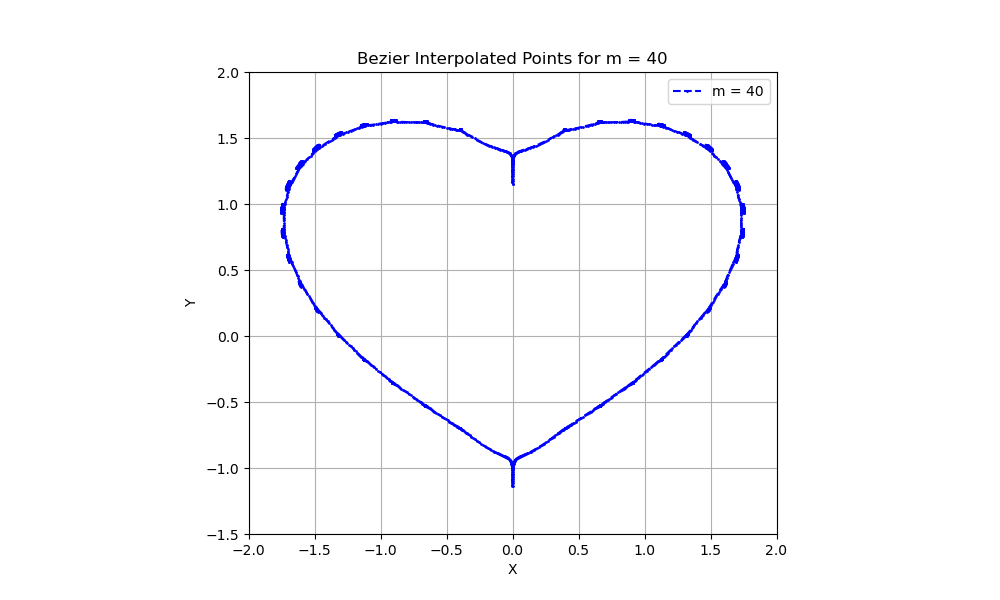
\includegraphics[width=\textwidth]{figures/bezier2.png}
    \caption{planar curve with m = 40}
    \label{fig:bezierm40}
  \end{minipage}
  \hfill
  \begin{minipage}[b]{0.45\textwidth}
    \centering
    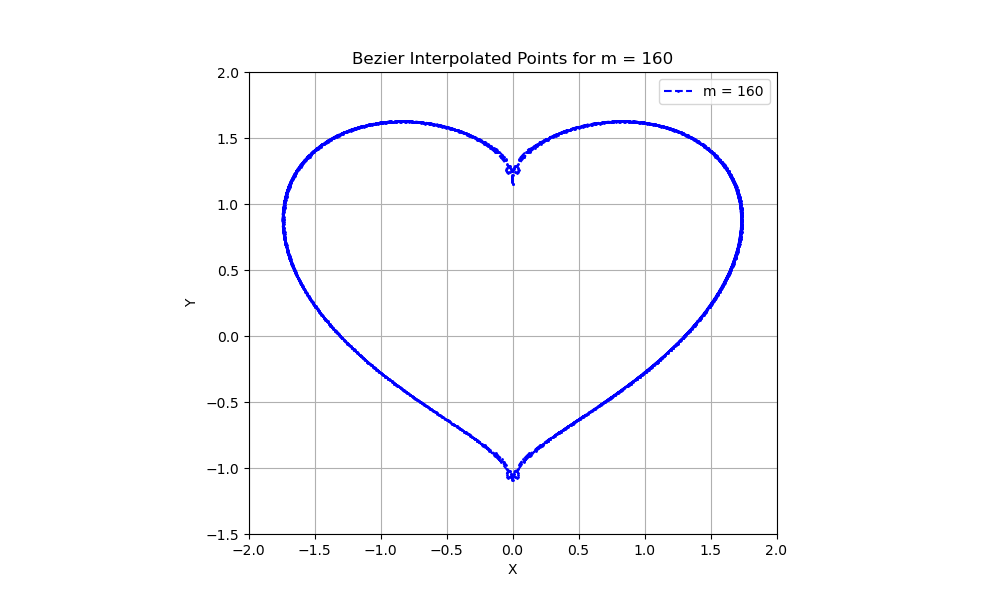
\includegraphics[width=\textwidth]{figures/bezier3.png}
    \caption{planar curve with m = 160}
    \label{fig:bezierm160}
  \end{minipage}
\end{figure}

From the figures, we can see that when \( m = 10 \), the original curve is already well-fitted. However, when \( m = 40 \), due to improper handling of the boundary conditions at the upper and lower endpoints, some issues appear at these points. When \( m = 160 \), the fitted curve almost perfectly matches the original curve.

Additionally, I selected the interpolation points uniformly according to the parameter \( t \), which is a relatively good choice. However, if the points were selected uniformly according to the curve length, better results could be obtained. Due to the difficulty of implementation, I did not achieve this.
% ===============================================
\section*{ \center{\normalsize {Acknowledgement}} }
The Python codes in the plotCode folder were largely generated with the assistance of ChatGPT.
\end{document}